\documentclass[a4paper]{article}
\usepackage[english]{babel}
\usepackage[utf8x]{inputenc}
\usepackage{amsmath}
\usepackage{graphicx}
\usepackage[colorinlistoftodos]{todonotes}
\usepackage{url}
\bibliographystyle{plain}
\title{Pseudo-random Number Generators: Linear and Non-linear Method}
\author{Donald Stevens}

\begin{document}
\maketitle

\begin{abstract}
Simulation and Modelling project: An attempt to create in the R programming language various kinds of pseudo-random number generators. Commentary regarding the endeavor included.\\

\noindent \textbf {keywords}
\begin {enumerate}
	\item Linear Congruential Generators (LCG)\\
	\item Multiple Recursive Generator (MRG)\\
	\item Combined LCGs and MRGs (CMRG)\\
	\item Inversive Congruential Generator (ICG)\\
	\item Quadratic Congruential Generators (QCG)\\
	\item Blum, Blum \& Shub generator (BBS)\\
\end {enumerate}
\end{abstract}

\section{Introduction}

There are two kinds of pseudo-random number generators in this paper, linear and non-linear. Their characteristics and limitations are discussed below. I will be using code samples made from within the R programming environment.

\section{Linear Pseudo-random Number Generation}
\label{sec:examples}

\subsection{Linear Congruential Generators (LCG)}

Using a linear equation one can produce a series of values that are reliably non-periodic. That is not easily distinguished repeated order of numbers will occur. The critical components to this generator are:
\begin{enumerate}
\item the "modulus" m
\item the "additive constant", or  c
\item the "multiplier" or a
\item and finally the "seed" or "start value" r0
\end{enumerate}

$$ r_{n + 1} = a \times r_n + c \pmod m $$

According to A. Gille-Genest, "The maximal period for a LCG is m. It is reached if and only if c is relatively prime to m, a - 1 is a multiple of p for every prime factor p of m and if m is a multiple of 4, then a - 1 is also a multiple of 4."\cite{Gille-Genest2014}

\subsection{Multiple Recursive Generators (MRG)}
For this paper I will be using the MRG described at the R-Project.Org\cite{Leydold2012}, specifically the generator, {\em rstream.mrg32k3a}

\begin{quote}The recurrence relation for a MRG is defined by:\\
	$x_n=(a_1 x_{n-1}\ldots +a_k x_{n-k}) \mod {m}$\cite{Gille-Genest2014}
\end{quote}

\subsection{Inversive Congruential Generators (ICG)}
defined by: $x_{n+1} = \overline{ax_n + b} \mod{m}$

\subsection{Quadratic Congruential Generators (QCG)}
described by Blum, Blum, and Shub: $g = a_1x_n^2+a_2x_n+c$

\subsection{Blum, Blum \& Shub Generator (BBS)}
defined as: $x_n=(x_{n-1})^{2} \mod {m}$, $x_0 = x_2 \mod {m}$ where ${m} = pq$ and p and q are both large prime numbers. The seed $x_0$ is greater than 1 and coprime to ${m}$, that is, it has no factors in common with p or q.
Additionally, p and q should be congruent to $3 \mod 4$. So the remainder of p divided by 4 and q divided by 4 is 3, as well as $x_0 / 4 = 3$
One you have done the square of $x_n-1 \mod {m}$ then calculate the least significant bit of the resulting $x_n$. The resulting calculation is your first random number.\cite{Menezes2010}


\subsection{Determining the PRNG performance measure.}
\par There are a few ways one can determine if the number set is random.
One simple method is simple to plot the numbers as seen in figures included and to observe the repetitive or cluster patterns seen in a non-random set. Some sets will converge to a single value over time, others will only appear random over a specific interval but beyond this interval the random pattern will recur, this is known as a lattice structure. For this reason picking the right prime numbers and constants is important.\cite{stata2014}
\par Currently, the best standard measure of randomness for a PRNG is the Dieharder series of tests by Robert G. Brown, Dirk Eddelbuettel, David Bauer from Duke University.\cite{Brown2014}
\par Following the example used by Strata for testing their random number generator, I first created a data set from each random number generator consisting of 3 million values in ascii format. Generally one would then convert it into hexadecimal and finally into binary as shown on their site, however it appears the current version of Dieharder can run the full suite of tests using a properly formatted ascii text file of numbers.\cite{stata2014}



% Commands to include a figure:
\begin{figure}
\centering
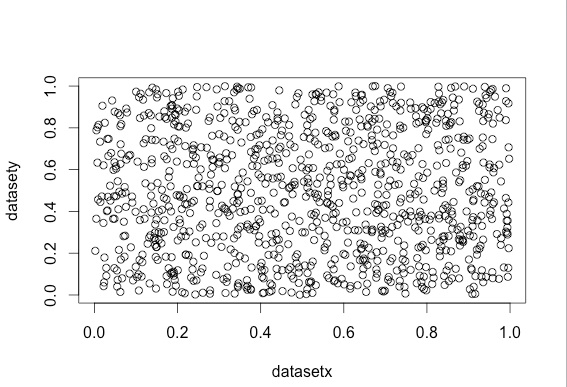
\includegraphics[width=0.95\textwidth]{plot.png}
\caption{\label{fig:plot}This figure shows two random datasets generated via Linear Congruential generation plotted as x,y coordinates between zero and one.}
\end{figure}

\begin{figure}
\centering
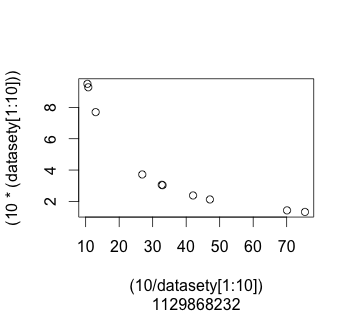
\includegraphics[width=0.60\textwidth]{Rplot1.png}
\caption{\label{fig:Rplot1}This figure shows a sample of 10 points plotted from datasety in the form (1/x,10x) using 1129868232 as the seed value.}
\end{figure}

\begin{table}
\centering
\begin{tabular}{l|r}
Number Generator & Dieharder Testing (sample size=3,000,000) \\\hline
LCG & 0.4259 \\
MRG & 0.0673 \\
CMRG & 1.2618 \\
ICG & 0.6254 \\
QCG & 13 \\
BBS & 13 \\
\end{tabular}
\caption{\label{tab:widgets}An example table.}
\end{table}

\LaTeX{} is great at mathematics. Let $X_1, X_2, \ldots, X_n$ be a sequence of independent and identically distributed random variables with $\text{E}[X_i] = \mu$ and $\text{Var}[X_i] = \sigma^2 < \infty$, and let
$$S_n = \frac{X_1 + X_2 + \cdots + X_n}{n}
      = \frac{1}{n}\sum_{i}^{n} X_i$$
denote their mean. Then as $n$ approaches infinity, the random variables $\sqrt{n}(S_n - \mu)$ converge in distribution to a normal $\mathcal{N}(0, \sigma^2)$.

\bibliography{prand_R_proj}
\end{document}